在我们理解了仿射概形后,射影概形\index{射影!概形}的理论并不会包含太多新奇的东西:在大多数情况下,它与射影簇的经典理论的差别完全类似于仿射概形和仿射簇的经典理论之间的差别。

我们首先将引入两个有限性条件,\textit{有限}以及\textit{有限型},然后定义和讨论\textit{分离}以及\textit{颇合}\footnote{译者注:将 proper morphism 译作“颇合态射”取自周健先生翻译的EGA.}态射\index{颇合!态射},它们分别对应于绝大多数几何中的Hausdorff性与紧性。而正是部分因为射影簇和概形有这些性质,它们才是经典代数几何以及概形理论的基本研究对象。

这章的下一部分将引入射影概形以及给出一些例子。如同仿射概形的情形,有两种入手射影概形的法子:一种是定义出射影空间然后取它们的子概形,另一种是将所有的射影概形建立在同一个根基上,从分次代数入手。正如处理仿射情况那般,这里我们采用第二种方法。

在介绍了射影概形的基础定义以及它们的子概形后,我们将描述射影概形之间的态射,相较于仿射对应,它将更加微妙而难以捉摸(就像在簇范畴中那样)。我们将用一些射影概形的例子结束这节,其中最值得注意的是Grassmannian.

本章的最后一节将给出嵌入在射影空间中的射影概形的三个不变量,它们由David Hilbert所引入:Hilbert多项式、Hilbert函数以及自由分解(free resolution). 使用它们,我们有时能区分类似的概形,比如射影双重直线,以及可以
揭示平坦性的一些新现象。在一个射影概形的不变量中,可以根据其Hilbert多项式定义的不变量的是它的度数;在这方面的联系,我们将讨论著名的B\'{e}zout定理。

\section{一些态射的性质}

\subsection{有限性条件}

在大多数有关概形的非平凡结论中,有两个有限性条件。它们有着相似的名字但非常不同的性质。第一个有限性条件,有限型,是一个在绝大多数几何背景中产生的态射都满足的直截了当的性质,他被引入常是为了排除无穷维的纤维或者“非几何”的概形,比如局部环的谱。而另一个有限性条件,有限,比较起来就是一个非常严格的条件:此时一个态射是颇合的以及它的所有纤维都是有限的(特别地,零维的)。

首先,我们称一个概形间的态射$\varphi:X\to Y$是\textit{有限型}的,如果对每一点$y\in Y$,都存在一个$y$的仿射开邻域$V=\spec B\subset Y$使得它的原像被一族仿射开集$U_i\cong \spec A_i$有限覆盖,即
\[
	\varphi^{-1}(V)=\bigcup_{i=1}^n U_i,
\]
并且在映射
\[
	\varphi_V^\#:B=\oo_Y(V)\to \oo_X (\varphi^{-1}V)\to \oo_X(U_i)=A_i
\]
下,每个$A_i$都是一个有限生成$B$\hyp 代数。因此,比如,任意$\mathbb{A}_K^n$或$\mathbb{P}_K^n$的子概形是在$K$上有限型的(意思是,结构态射$X\to \spec K$是有限型的),而一个正维数的局部$K$\hyp 代数的谱不是。

一个态射$\varphi:X\to Y$被称为\textit{有限}\index{有限}的,如果对每点$y\in Y$都有它的一个开仿射邻域$V=\spec B\subset Y$使得原像$\varphi^{-1}(V)=\spec A$也是仿射的,以及通过拉回
\[
	\varphi_X^\#L: B =\oo_Y(V)\to \oo_X(\varphi^{-1}V)=A,
\]
$A$是一个有限生成$B$-模。这是一个比有限型更强的条件,首先,马上可以由其给出$\varphi$的纤维是有限的,其次,拓扑空间之间的映射$|\varphi|:|X|\to |Y|$是一个闭映射。因此,对$Y=\spec B$以及多项式$f\in B[x]$,如果$f$的最高项系数是一个可逆元,则态射$\varphi(B[x]/(f))\to Y$是有限的。这些都可以参考 Eisenbud [1995, Chapter 4 and Section 9.1].

\subsection{颇合性和分离性}

许多几何上的技术应用于紧Hausdorff空间时可以获得最完整的结果。尽管仿射概形在Zariski拓扑下是预紧的,但是它们并不共享在其他理论中紧空间的良好属性,因为Zariski拓扑不是Hausdorff的。举个例子,即使X是预紧的,仿射概形间的正则映射$\varphi:X\to Y$的像也可能不是闭的。

Zariski拓扑并不Hausdorff这点还有着其他令人不爽的结果。回忆在流形的一般定义中,我们从一个Hausdorff空间开始,在它上面装备一个坐标卡的覆盖,坐标卡是一个标准型(即欧式空间中的球)。但注意到,即使这些球都是Hausdorff的,也不足以说明整个空间是Hausdorff的。这就是为什么在Exercise \ref{exe:1.44}中描述的具有双重原点的直线(这里重新展示如下)

\begin{center}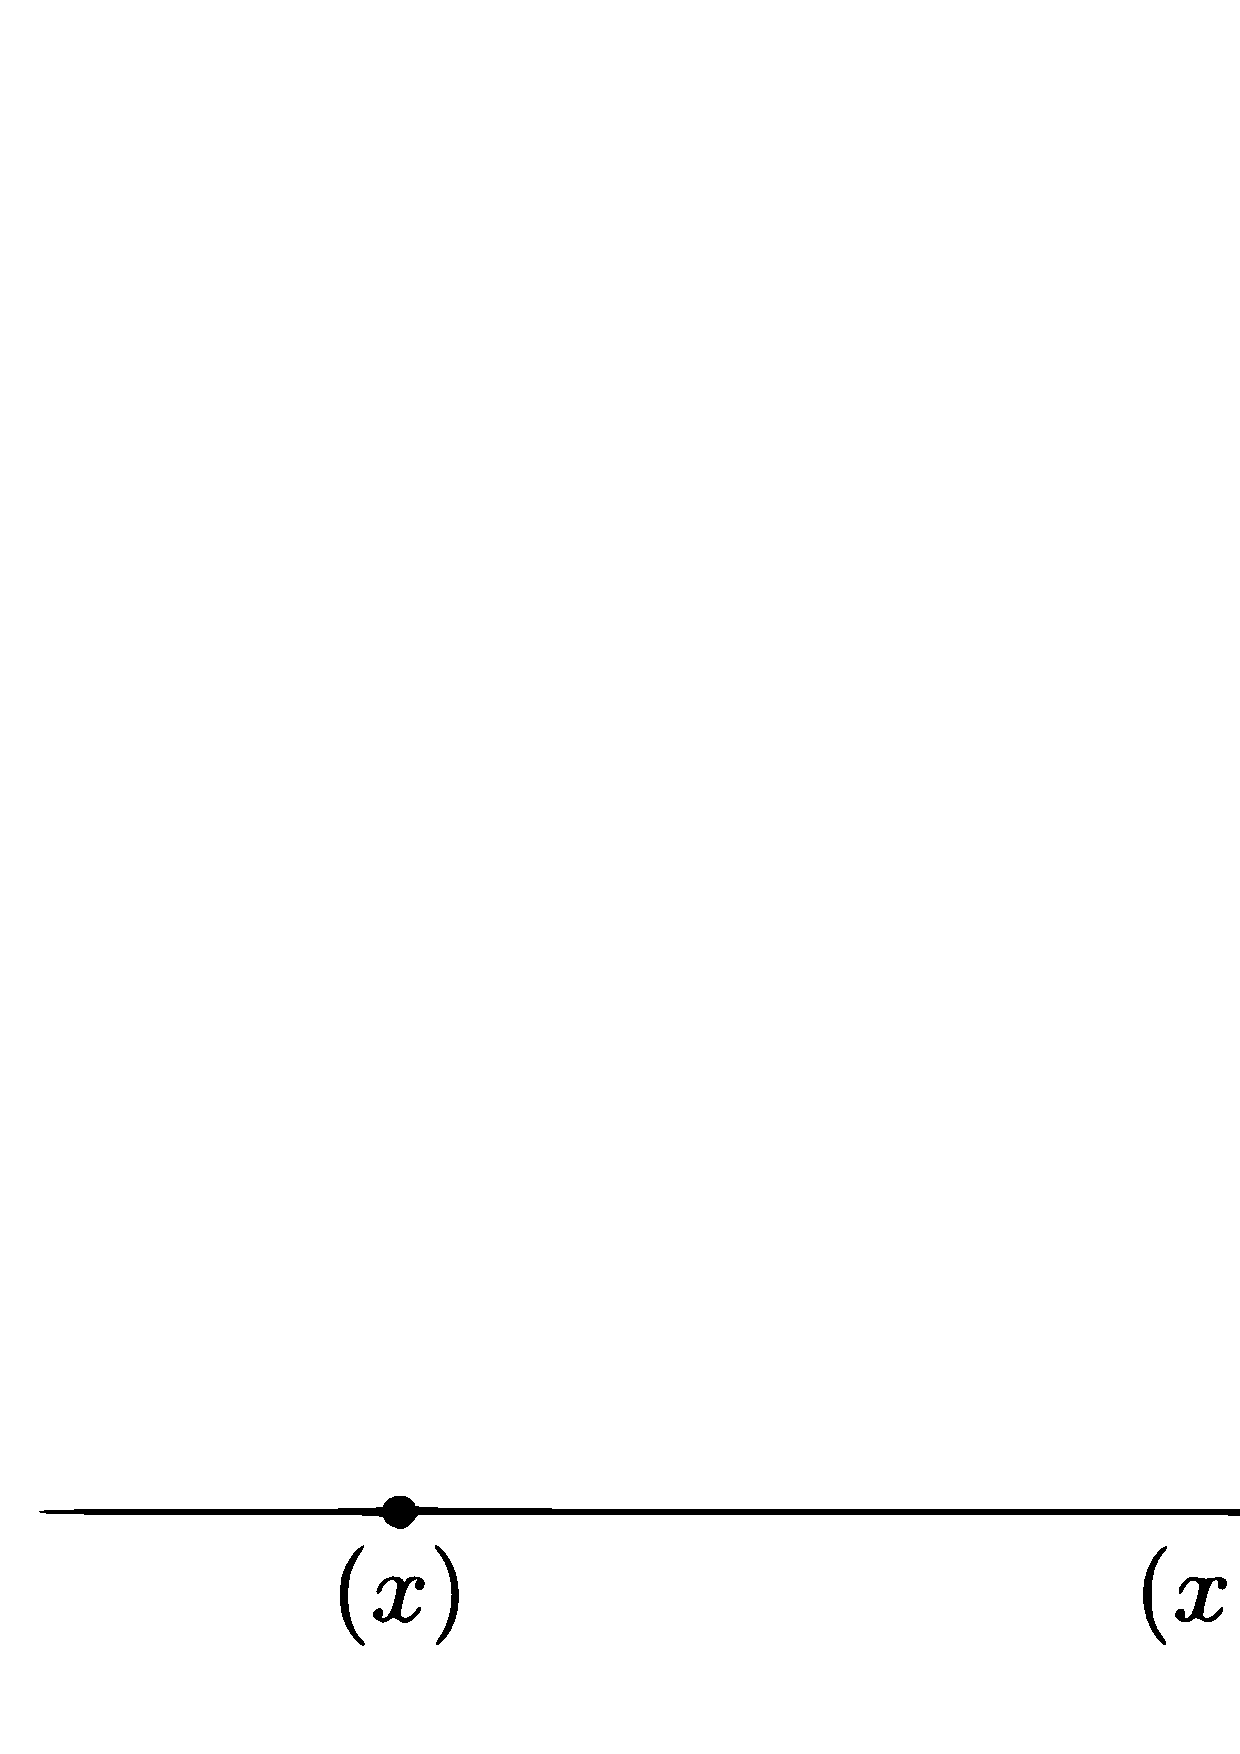
\includegraphics[scale=\scale,bb=0 0 562 68]{chap_3/pics/1.png}\end{center}

\vspace{-0.4em}\noindent 不是一个流形。然而,当我们处理由仿射概形拼成的概形(或者簇)的时候,我们不能指定整个空间是Hausdorff的,因为即使就局部来说,那些拼合的部件也不是Hausdorff的。于是,对给定两个概形之间的两个态射$\varphi$, $\psi:X\to Y$,$\varphi$和$\psi$相等的点构成的集并不会是闭的。下面习题中的典型例子将展示这点。

\begin{exe}
\begin{compactenum}[(a)]
\item 令$Y$是在域$K$上的具有双重原点的直线,正如在Exercise \ref{exe:1.44}中定义的那样,以及令$\varphi_1$, $\varphi_2:\mathbb{A}_K^1\to Y$是两个显然的含入映射,证明$\varphi_1$和$\varphi_2$相等的点(仅作为拓扑空间间的连续映射)构成的集合不是闭的。
\item 现在令$X=Y\times_K Y$以及$\varphi$和$\psi$是两个到$X$到$Y$的投射。证明,$\varphi$和$\psi$相等的点构成的集合不是闭的。证明,使得$\varphi$和$\psi$相等的闭点构成的集合也不是闭的。所以这个病态现象并不是概形特有的,它在簇的范畴中已经出现了。
\end{compactenum}
\end{exe}

如果$X$是一个仿射概形,这样的病态现象并不会出现,反之,当$X$是一个射影概形的时候,它将会出现。

\[
	X\supset \spec A\xrightarrow{\alpha|_{\spec A}}\spec B\subset S
\]
